\documentclass[crop, tikz]{standalone}

\usepackage[utf8]{inputenc}
% 'crop' is the default for v1.0, before it was 'preview'
%\usetikzlibrary{...}% tikz package already loaded by 'tikz' option

\usetikzlibrary{arrows}
\usetikzlibrary{decorations.markings}

\begin{document}

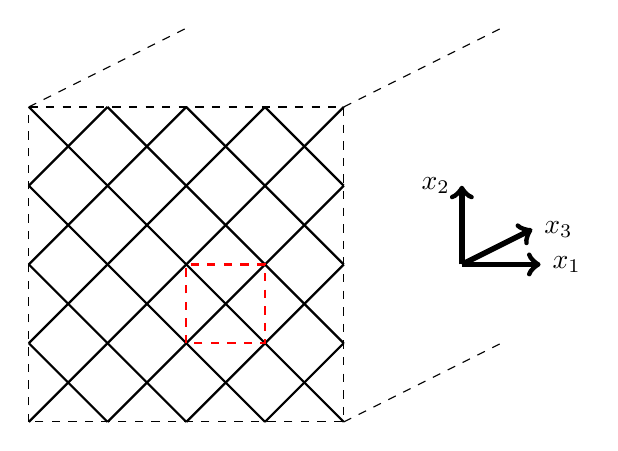
\begin{tikzpicture}

	%x_1,x_2-plane with period cell highlighted
	\draw[dashed] (0,0) rectangle (4,4);	
	%x_3 fibre axes effect
	\draw[dashed] (4,4) -- (6,5);
	\draw[dashed] (4,0) -- (6,1);
	\draw[dashed] (0,4) -- (2,5);

	%pattern filling the x1-x2 plane
	%BL-TR
	\draw[thick, black] (0,3) -- (1,4);
	\draw[thick, black] (0,2) -- (2,4);
	\draw[thick, black] (0,1) -- (3,4);
	\draw[thick, black] (0,0) -- (4,4);
	\draw[thick, black] (1,0) -- (4,3);
	\draw[thick, black] (2,0) -- (4,2);
	\draw[thick, black] (3,0) -- (4,1);
	%BR-TL
	\draw[thick, black] (0,4) -- (4,0);
	\draw[thick, black] (0,3) -- (3,0);
	\draw[thick, black] (0,2) -- (2,0);
	\draw[thick, black] (0,1) -- (1,0);
	\draw[thick, black] (1,4) -- (4,1);
	\draw[thick, black] (2,4) -- (4,2);
	\draw[thick, black] (3,4) -- (4,3);
	
	%unit cell outline
	\draw[thick, red, dashed] (2,1) rectangle (3,2);
	
	%co-ordinate axes
	\begin{scope}[scale=1.0, shift={(5.5,2)}]
		\draw[->, line width=2.0] (0,0) -- (1,0) node[anchor=west] {$x_1$};
		\draw[->, line width=2.0] (0,0) -- (0,1) node[anchor=east] {$x_2$};
		\draw[->, line width=2.0] (0,0) -- ({2/sqrt(5)}, {1/sqrt(5)}) node[anchor=west] {$x_3$};
	\end{scope}

\end{tikzpicture}

\end{document}